% ============================================================
%  Chapter 2: Background
% ============================================================
%
% AIM: Establish the mathematical and physical foundations for CT
%      reconstruction. A reader who finishes this chapter should
%      understand the forward model, why inversion is hard, and what
%      classical algorithms do. No ML yet -- that is Chapter 3.
%      ~6-8 pages.
%
% CONTENTS:
%   2.1 CT Physical and Mathematical Foundations
%       - Beer-Lambert law (Eq. for attenuation)
%       - Line integrals and the sinogram
%       - Continuous Radon transform (definition, notation)
%       - Central Slice Theorem (statement, no proof)
%       - Discrete forward model y = Ax + eta
%       - Remark on LION/tomosipo operator abstraction
%
%   2.2 Ill-Posedness of the CT Inverse Problem
%       - Hadamard conditions
%       - Sparse-view: undersampled angles, null space, streak artefacts
%       - Limited-angle: directional blurring
%       - Noise amplification: ramp filter, SVD decay
%       - Noise model: Poisson -> Gaussian after log transform
%       - Connection to TFPnP noise levels (5%, 7.5%, 10%)
%
%   2.3 Classical Reconstruction Algorithms
%       - FBP: filter then backproject, exact under ideal conditions
%       - SIRT: iterative least-squares, gradient descent with scaling
%       - TV minimisation: piecewise-constant prior, PDHG solver
%       - Brief comparison of strengths/weaknesses
%
%   2.4 From Classical to Learned: A Bridge
%       - What classical methods lack (data-driven priors)
%       - The key question: can we learn the prior from data?
%       - Pointer to Chapter 3
%
% FIGURES:
%   - Fig 2.1: CT acquisition geometry diagram (parallel beam)
%              [Create in TikZ or export from tomosipo notebook]
%   - Fig 2.2: Example sinogram and its FBP reconstruction
%              [Generate from tomosipo notebook]
%   - Fig 2.3: Sparse-view artefacts: FBP with 720 vs 30 views
%              [Generate from tomosipo notebook]
%   - Fig 2.4: TV reconstruction of same sparse-view data
%              [Generate from tomosipo notebook]
%
% CITATIONS NEEDED:
%   Radon 1917, Natterer 2001, Hadamard 1923, Herman 2009,
%   Buzug 2008, Gilbert 1972, Rudin-Osher-Fatemi 1992,
%   Sidky-Pan 2008, Chambolle-Pock 2011, Feldkamp 1984,
%   Hansen 1992/1998, Biguri 2016 (TIGRE)
% ============================================================

\chapter{Background}
\label{chap:background}

This chapter establishes the mathematical and physical foundations required to understand
learned reconstruction methods for computed tomography (CT). We begin with the
X-ray physics and the forward model, move to a careful treatment of ill-posedness, and
conclude with a survey of the classical reconstruction algorithms that serve as baselines
throughout this project.

% -----------------------------------------------------------
\section{Computed Tomography: Physical and Mathematical Foundations}
\label{sec:ct-basics}
% -----------------------------------------------------------

\subsection{X-ray Attenuation and the Beer--Lambert Law}

When a monochromatic X-ray beam of initial intensity $I_0$ traverses a material along
a straight line $L$, photons are absorbed and scattered by the medium. The local
probability of an interaction per unit length is described by the \emph{linear attenuation
coefficient} $\mu(\bm{x}) \geq 0$, which depends on both tissue composition and photon
energy. The Beer--Lambert law governs the transmitted intensity $I$:
\begin{equation}
    I = I_0 \exp\!\left(-\int_L \mu(\bm{x})\,\mathrm{d}\ell\right),
    \label{eq:beer-lambert}
\end{equation}
where $\ell$ parameterises arc length along the ray. Taking logarithms, one obtains the
\emph{line integral} (or projection):
\begin{equation}
    p = -\ln\!\left(\frac{I}{I_0}\right) = \int_L \mu(\bm{x})\,\mathrm{d}\ell.
    \label{eq:line-integral}
\end{equation}
In practice, $\mu$ is the unknown quantity one wishes to recover; $p$ is measurable for
each ray. A full CT acquisition collects such integrals over many lines, indexed by angle
$\phi$ and detector position $s$, forming the \emph{sinogram}.

% TODO: Add Figure 2.1 here -- CT acquisition geometry diagram
% \begin{figure}[htbp]
%     \centering
%     \includegraphics[width=0.7\textwidth]{figures/ct_geometry.pdf}
%     \caption{Parallel-beam CT acquisition geometry.}
%     \label{fig:ct-geometry}
% \end{figure}

\subsection{The Continuous Radon Transform}

The mathematical abstraction of the projection process is the \emph{Radon transform}
\citep{Radon1917}. For a function $f : \mathbb{R}^2 \to \mathbb{R}$ (representing the
attenuation map), the Radon transform $\mathcal{R}$ is defined as:
\begin{equation}
    (\mathcal{R}f)(\phi, s)
        = \int_{-\infty}^{\infty} f\!\left(s\bm{\theta} + t\bm{\theta}^{\perp}\right)\mathrm{d}t,
    \label{eq:radon}
\end{equation}
where $\bm{\theta} = (\cos\phi, \sin\phi)^T$ is the unit vector in the projection direction,
$\bm{\theta}^{\perp} = (-\sin\phi, \cos\phi)^T$ is orthogonal to it, and $s \in \mathbb{R}$ is the
signed distance from the origin to the line. The domain of $(\phi, s)$ is called the
\emph{sinogram domain} or \emph{Radon domain}. For a three-dimensional object, the
corresponding transform integrates over planes rather than lines; in fan-beam or
cone-beam geometries the lines emanate from a single source point, yielding a modified
geometry \citep{Natterer2001}.

A key analytical result is the \emph{Central Slice Theorem} (also called the Fourier Slice
Theorem): the one-dimensional Fourier transform of a projection at angle $\phi$ equals
a radial slice of the two-dimensional Fourier transform of $f$ at the same angle. This
relationship underpins the filtered backprojection algorithm described in
\cref{sec:classical-reconstruction}.

\subsection{The Discrete Forward Model}

Physical CT systems are digital: the detector has a finite number of pixels, the source
rotates to a finite set of angles, and the reconstructed image is represented on a grid.
After discretisation, the continuous relation \eqref{eq:radon} becomes a large linear
system. Let $\bm{x} \in \mathbb{R}^n$ be the vectorised image (pixel values of the attenuation map
arranged in raster order) and $\bm{y} \in \mathbb{R}^m$ be the vector of all measured line integrals
(the sinogram, row-stacked). The \emph{forward model} is:
\begin{equation}
    \bm{y} = A\bm{x} + \bm{\eta},
    \label{eq:forward-model}
\end{equation}
where $A \in \mathbb{R}^{m \times n}$ is the \emph{system matrix} (or \emph{projection matrix})
whose entry $A_{ij}$ encodes the contribution of pixel $j$ to measurement $i$---typically
the length of the intersection of ray $i$ with pixel $j$---and $\bm{\eta}$ represents
additive noise. This is the fundamental model throughout the project; the goal of
reconstruction is to recover $\bm{x}$ from $\bm{y}$ and $A$.

\begin{remark}
In the LION/tomosipo framework used in this project \citep{Biguri2016TIGRE}, $A$ is
never stored explicitly---it would be $\mathcal{O}(mn)$ in memory for large volumes---but is
instead evaluated on-the-fly via GPU-accelerated forward and back-projection operators.
The linear map $A$ and its adjoint $A^T$ (the \emph{backprojection} operator) are
therefore available as callable functions rather than dense matrices.
\end{remark}

\begin{figure}[htbp]
    \centering
    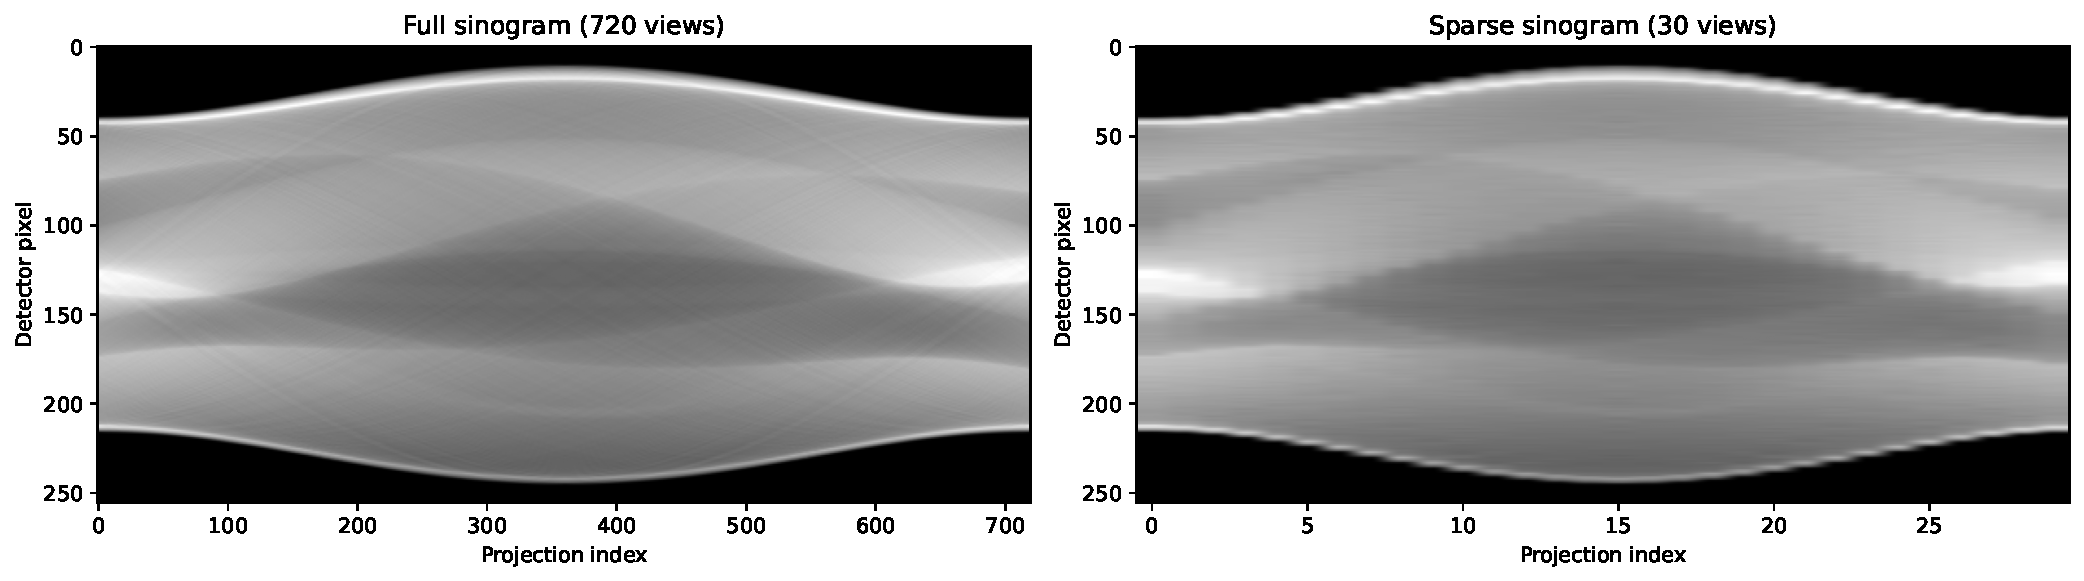
\includegraphics[width=\textwidth]{figures/sinogram_comparison.pdf}
    \caption{Sinogram comparison for the Shepp-Logan phantom. \textbf{Left}: full sinogram
             with 720 projection angles (the clinical standard). \textbf{Right}: sparse
             sinogram with only 30 angles, corresponding to a $24\times$ dosage reduction.
             The sparse sinogram contains the same sinusoidal structure but sampled at
             far fewer angular positions, leaving large gaps in the Radon domain.}
    \label{fig:sinogram-comparison}
\end{figure}

% -----------------------------------------------------------
\section{Ill-Posedness of the CT Inverse Problem}
\label{sec:ill-posedness}
% -----------------------------------------------------------

Recovering $\bm{x}$ from $\bm{y}$ is an \emph{inverse problem}. When measurements are
complete and noise-free, the Radon transform is invertible (via the classical inversion
formula); however, practical CT acquisition violates both conditions, rendering the
problem ill-posed in the sense of Hadamard \citep{Hadamard1923}: solutions may not
exist, may not be unique, or may not depend continuously on the data.

\subsection{Sources of Ill-Posedness}

\paragraph{Sparse-view CT.}
To reduce patient radiation dose---the primary concern motivating this project---one
reduces the number of projection angles. The Mayo Clinic Low Dose CT Grand Challenge
dataset \citep{MayoClinic} provides a canonical low-dose benchmark. When the number of
angles drops below the Nyquist-like sampling criterion (informally: at least $(\pi/2)N$
views for an $N \times N$ image), the sinogram is severely undersampled. Analytically,
the null space of the undersampled $A$ is non-trivial: many images $\bm{x}$ yield the
same measurements $\bm{y}$, so the problem is underdetermined ($m \ll n$). The artefacts
produced by naive reconstruction are radially symmetric streak artefacts aligned with
the missing-angle directions.

\paragraph{Limited-angle CT.}
A related but distinct scenario arises when projections are available only over a
restricted angular range (e.g., $[0\degree, 120\degree]$). In tomosynthesis and some industrial
settings this is unavoidable due to geometry constraints. Here the null space of $A$
contains low-frequency components aligned with the missing angular sector, producing
characteristic directional blurring.

\paragraph{Noise amplification.}
Even with a full set of angles, the continuous Radon inversion formula amplifies
high-frequency noise: it involves differentiation (the ramp filter in FBP), which
multiplies Fourier coefficients by $|\xi|$, the spatial frequency. Consequently, white
measurement noise $\bm{\eta}$ leads to high-frequency artefacts in naively inverted
images. Physically, quantum (Poisson) noise in the photon counts is the dominant
source \citep{Buzug2008}.

\paragraph{Formal characterisation.}
The singular value decomposition (SVD) of $A$ reveals the mechanism: the singular
values $\sigma_i$ of $A$ decay, often rapidly, towards zero. Inverting $A$ via
$\bm{x} = A^+ \bm{y}$ (the pseudoinverse) amplifies the components of $\bm{y}$ lying in the
direction of small singular vectors by $1/\sigma_i$, which diverges as
$\sigma_i \to 0$. This is the hallmark of a \emph{discrete ill-posed problem}
\citep{Hansen1992,Hansen1998}.

\begin{figure}[htbp]
    \centering
    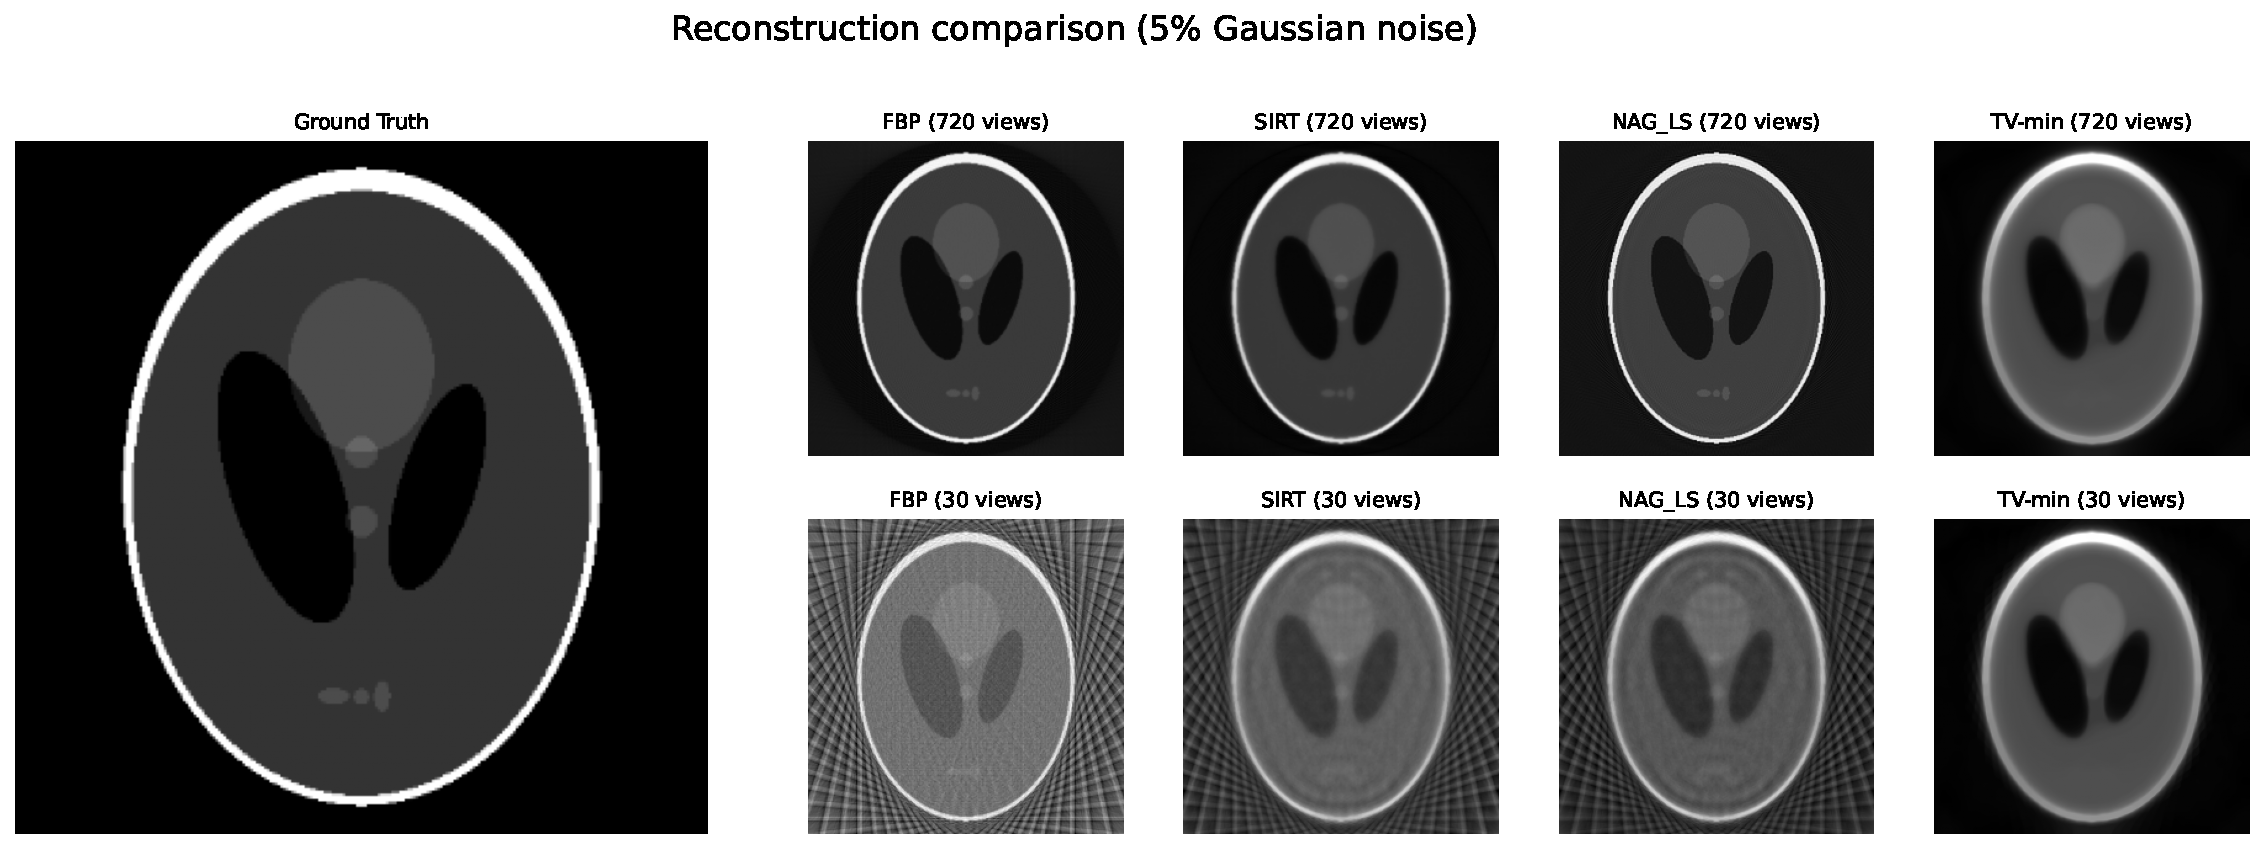
\includegraphics[width=\textwidth]{figures/reconstruction_comparison.pdf}
    \caption{Reconstruction comparison on the Shepp-Logan phantom with 5\% Gaussian noise.
             \textbf{Top row}: ground truth, FBP from 720 views (clinical reference), and
             FBP from 30 views (severe streak artefacts). \textbf{Bottom row}: SIRT, NAG\_LS,
             and TV minimisation, all from 30 views. The degradation from 720 to 30 views
             in FBP illustrates the ill-posedness of the sparse-view problem.}
    \label{fig:reconstruction-comparison}
\end{figure}

\subsection{Noise Model}

The physical acquisition process introduces Poisson-distributed noise in the photon
counts. After the log-transformation \eqref{eq:line-integral}, the sinogram noise is
approximately Gaussian for moderate dose levels (by the central limit theorem) and
can be written:
\begin{equation}
    \bm{\eta} \sim \mathcal{N}(\bm{0}, \sigma^2 I),
\end{equation}
where $\sigma^2$ depends on dose level. In the sparse-view CT experiments of the TFPnP
paper \citep{Wei2022TFPnP}, Gaussian noise with levels $\sigma \in \{5\%, 7.5\%, 10\%\}$
is added to the projections after the Radon transform, simulating realistic low-dose
acquisition at a $24\times$ dosage reduction compared to the 720-view standard.


% -----------------------------------------------------------
\section{Classical Reconstruction Algorithms}
\label{sec:classical-reconstruction}
% -----------------------------------------------------------

Before learned methods, three families of algorithms dominated CT reconstruction.
These serve as baselines in the experimental evaluation and underpin the learned methods
reviewed in \cref{chap:related-work}.

\subsection{Filtered Backprojection (FBP)}

Filtered backprojection is the standard clinical workhorse, derived analytically from the
inversion of the continuous Radon transform via the Central Slice Theorem. The algorithm
proceeds in two stages:

\begin{enumerate}
    \item \textbf{Filtering.} Each projection $p(\phi, \cdot)$ is convolved in the $s$-domain
          with a \emph{ramp filter} $h(s)$ whose Fourier transform is $|\xi|$, compensating
          for the non-uniform density of Fourier samples:
          \[
              \tilde{p}(\phi, s) = \bigl(p(\phi, \cdot) * h\bigr)(s).
          \]
    \item \textbf{Backprojection.} The filtered projections are smeared back into image space
          by integrating over all angles:
          \[
              f(\bm{x}) = \int_0^{\pi} \tilde{p}\!\left(\phi,\, \bm{x}\cdot\bm{\theta}\right)\mathrm{d}\phi.
          \]
\end{enumerate}

FBP is exact in the limit of dense, noiseless, full-angle sampling. Its principal
shortcomings are: (i) the ramp filter amplifies high-frequency measurement noise,
requiring an apodisation window (e.g., Hann, Ram-Lak) that blurs fine structures;
(ii) streak artefacts appear under sparse-view sampling. For cone-beam geometry, the
Feldkamp--Davis--Kress (FDK) algorithm \citep{Feldkamp1984} extends FBP and is
available in LION as \texttt{fdk}.

\subsection{Simultaneous Iterative Reconstruction Technique (SIRT)}

Iterative algebraic methods treat reconstruction as a least-squares problem:
\begin{equation}
    \min_{\bm{x}} \frac{1}{2}\|\,A\bm{x} - \bm{y}\,\|_2^2.
    \label{eq:least-squares}
\end{equation}
SIRT \citep{Gilbert1972} approximates the solution via gradient descent with a scaled step:
\begin{equation}
    \bm{x}^{(k+1)} = \bm{x}^{(k)} + C A^T R\!\left(\bm{y} - A\bm{x}^{(k)}\right),
\end{equation}
where $C = \operatorname{diag}(1/\sum_i A_{ij})$ and $R = \operatorname{diag}(1/\sum_j A_{ij})$
are diagonal scaling matrices (column and row sums of $A$) that normalise the step and
ensure convergence. SIRT converges to the minimum $\ell^2$-norm least-squares solution.
It handles missing data more gracefully than FBP (no explicit ramp amplification), but
converges slowly and is still unstable in the presence of noise without early stopping or
regularisation. LION provides a differentiable implementation via
\texttt{ts\_algorithms.SIRT}.

\subsection{Total Variation Minimisation}

Motivated by the observation that medical CT images are approximately piecewise constant
(and thus have sparse gradients), \citet{RudinOsherFatemi1992} introduced the
\emph{total variation} (TV) regulariser:
\begin{equation}
    \mathrm{TV}(\bm{x}) = \|\nabla \bm{x}\|_1
        = \sum_{i,j} \sqrt{|\partial_x x_{ij}|^2 + |\partial_y x_{ij}|^2},
\end{equation}
and \citet{SidkyPan2008} applied it to CT reconstruction as:
\begin{equation}
    \min_{\bm{x} \geq 0}\;\mathrm{TV}(\bm{x})
        \quad \text{subject to} \quad \|A\bm{x} - \bm{y}\|_2 \leq \varepsilon,
    \label{eq:tv-min}
\end{equation}
where $\varepsilon$ bounds the noise level. This is a convex optimisation problem solvable
by primal-dual splitting methods, such as the Primal-Dual Hybrid Gradient (PDHG) algorithm
of \citet{ChambolleAndPock2011}, available in LION as \texttt{tv\_min}. TV
reconstruction produces visually clean images with preserved edges, but can introduce
the characteristic \emph{staircase artefact} and requires careful selection of $\lambda$
(or equivalently $\varepsilon$). In the TFPnP sparse-view CT experiments, TV with
optimally tuned parameters achieves 20.91/19.17/16.95\,dB PSNR for the three noise
levels---substantially above FBP but below learned methods \citep{Wei2022TFPnP}.

\begin{figure}[htbp]
    \centering
    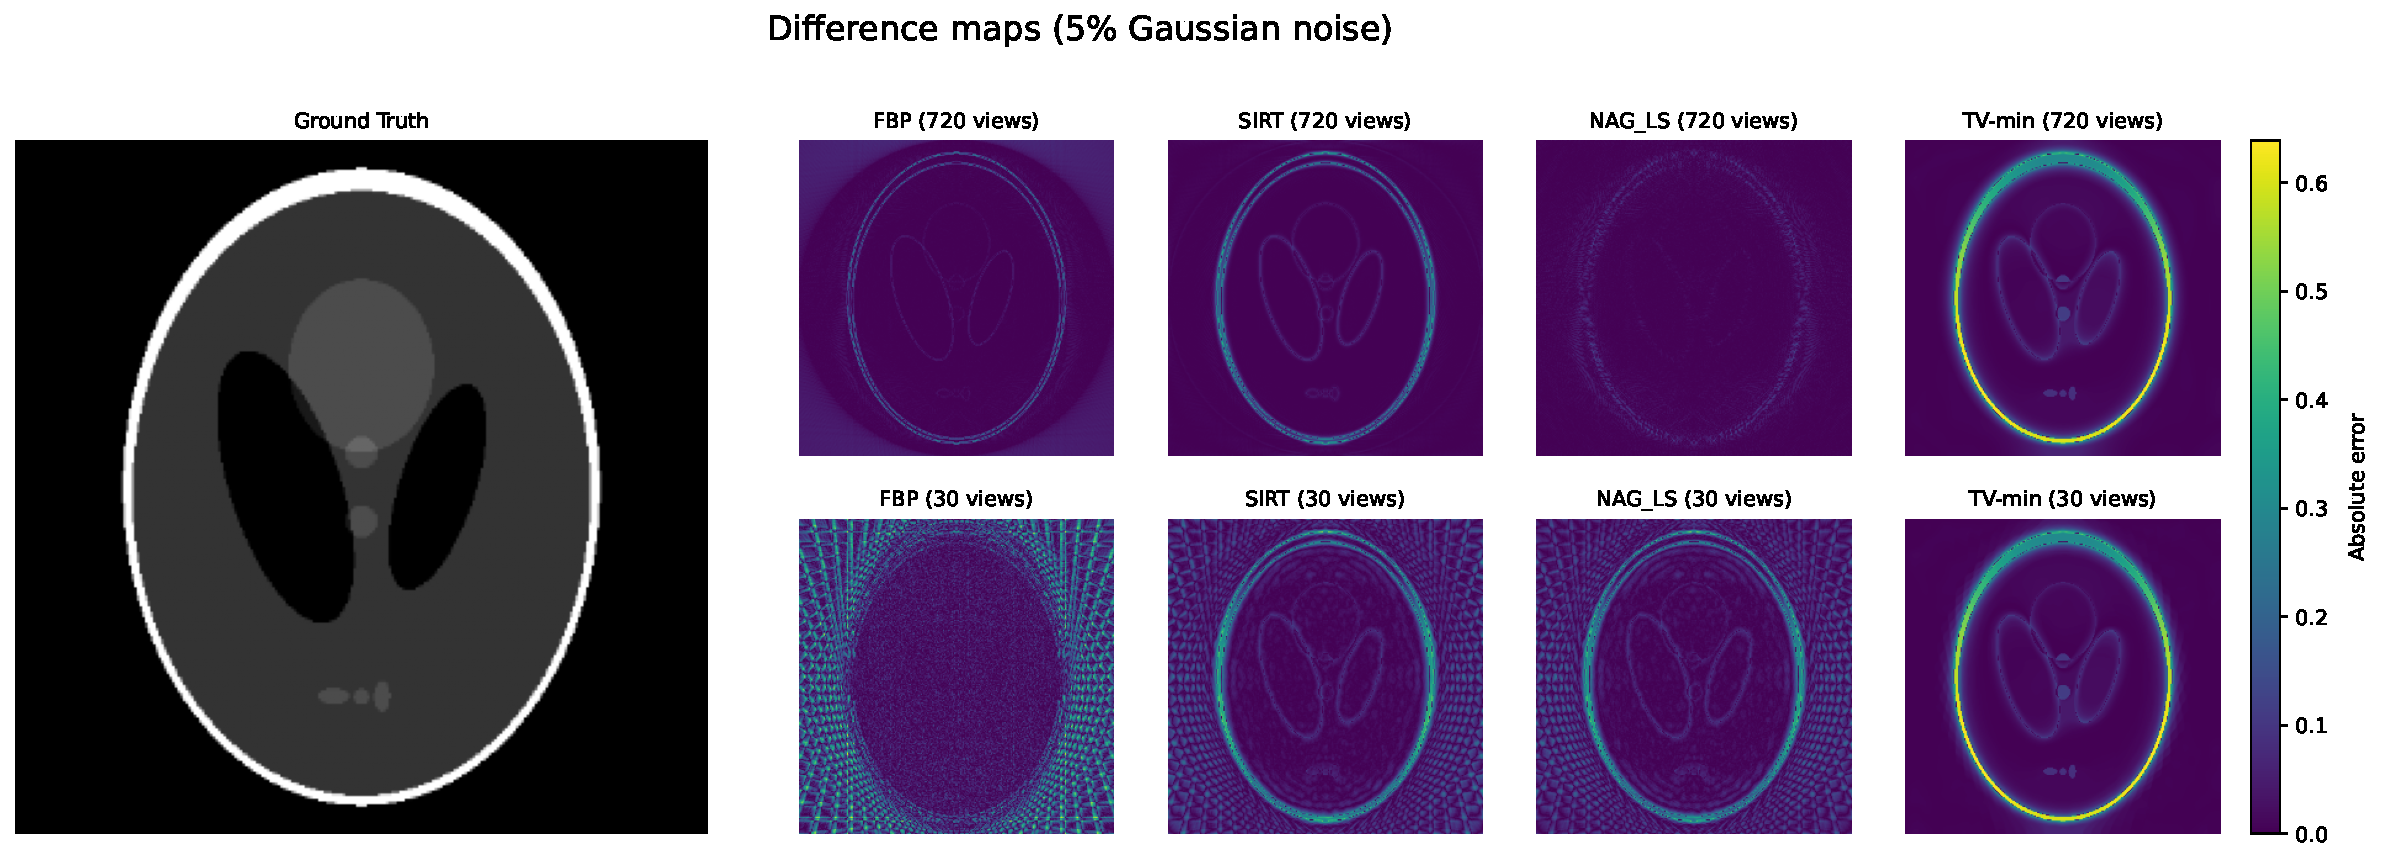
\includegraphics[width=\textwidth]{figures/difference_maps.pdf}
    \caption{Difference maps $\hat{\bm{x}} - \bm{x}^*$ for three reconstruction methods
             from 30-view sparse sinograms with 5\% noise. \textbf{Left}: FBP shows
             structured streak artefacts (correlated error). \textbf{Centre}: SIRT shows
             diffuse error concentrated at edges. \textbf{Right}: TV minimisation achieves
             the lowest error overall but shows sharp transitions at edges characteristic
             of the staircase artefact.}
    \label{fig:difference-maps}
\end{figure}

\subsection{From Classical to Learned: A Bridge}
\label{sec:bridge}

The fundamental limitation of both FBP and iterative methods is that they either
(a) invert the forward model analytically without data-driven priors (FBP), or
(b) assume a hand-crafted regulariser such as TV whose inductive bias may not align with
the true distribution of CT images. The key question motivating the field of learned
reconstruction is: \emph{can we replace or supplement the hand-crafted prior with one
learned directly from data?} \Cref{chap:related-work} surveys the spectrum of approaches
that have emerged to address this question---from variational regularisation through deep
unrolling to plug-and-play methods---culminating in TFPnP, the method implemented in
this project.